%!TEX root = /Users/louis/Documents/PhD/Deliverables/Thesis/thesis.tex

\chapter{Evaluation}
\label{Evaluation}

%The evaluation chapter will outline our evaluation method and results, including the impact and limitations of our research; and discuss the extent to which the requirements identified in the analysis chapter have been fulfilled. Evaluation will be conducted in three ways: application of our structures and processes in a case study; publication of our research in academic journals, international conferences and workshops; and assessing the contribution made when delivering our work through an Eclipse research incubation project.

\section{Evaluation Measures}

\subsection{Case Study}
% We will apply our structures and processes to the Eclipse Generative Modelling Framework (GMF) project \cite{gronback06gmf}. GMF allows the definition of graphical concrete syntax for metamodels. GMF prescribes a model-driven approach: Users of GMF define concrete syntax as a model, which is used to generate a graphical editor. In fact, five models are used together to define a single editor using GMF.

% GMF defines the metamodels for graphical, tooling and mapping definition models; and for generator models. The metamodels have changed considerably during the development of GMF. Some changes have caused inconsistency with GMF models. Presently, migration is encoded in Java. Gronback has stated\footnote{Private communication, 2008.} that the migration code is being ported to QVT (a model-to-model transformation language) as the Java code is difficult to maintain.

% We identified GMF as the most appropriate candidate for the analysis phase of our research. Consequently, we decided to reserve GMF for the evaluation of our work.


\subsection{Collaborative Case Study}

\subsection{Transformation Tools Contest}



\subsection{Quantitive Comparison of Model Migration Languages}
As discussed in Chapter~\ref{Implementation}, the languages currently used for model migration vary. Model-to-model transformation languages are used in some migration tools (e.g. \cite{cicchetti,garces}); general-purpose languages in others (e.g. \cite{ecore2ecore,cope}) and in ad-hoc solutions to migration (e.g. \cite{gmf}).

In developer-driven migration, a programming language codifies the migration strategy. Because migration involves deriving the migrated model from the original, migration strategies typically access information from the original model and, based on that information, update the migrated model in some way. As such, migration is written in a language with constructs for accessing and updating the original and migrated models. Here, those language constructs are termed \textit{model operations}. Using XX examples of model migration, this section explores the variation in frequency of \emph{model operation} over different model migration languages, and discusses to what extent the results of this comparison can be used to assess the suitability of the languages considered for model migration.

The remainder of this section.... TODO


\subsection{Method}
XX examples of co-evolution, taken from the projects identified in Chapter~\ref{Analysis}, were used to explore the variation in frequency of model operations over different migration languages. For each example, a migration strategy was written in each migration language to be compared. The correctness of the migration strategy was assured by comparing the migrated models provided by the co-evolution example with the result of executing the migration strategy on the original models provided by the co-evolution example.

For each migration language, a set of model operations were identified, as described in Section~\ref{subsec:model_migration_languages}. A program was written to count the number of \emph{model operations} appearing in each migration strategy. The results are presented in Section~\ref{subsec:quantitive_results}.

There are two non-trivial threats to the validity of the comparison performed in this section. Firstly, the author wrote the migration strategies for Epsilon Flock (a migration language that the author developed) and for the other migration languages considered (which the author has not developed). Therefore, it is possible that the migration strategies written in the latter may contain more model operations than necessary. For some migration languages, it was possible to reduce the effects of this threat by re-using or adapting existing migration strategy code written by the migration language authors. This is discussed further in Section~\ref{model_migration_languages}.

Secondly, the examples of co-evolution used to perform this analysis were taken from Chapter~\ref{Analysis} and have influenced the development of Flock, as discussed in Chapter~\ref{Implementation}.  % To mitigate this, could I perform the comparison again on GMF, UML, etc?


\subsection{Model Migration Languages}
\label{subsec:model_migration_languages}
The variation in frequency of model operations was explored across three model migration languages, ATL (used in  \cite{cicchetti,garces}), Groovy (as used in \cite{cope}), and Epsilon Flock, the migration language developed in this thesis. Here, the model operations of each language are identified. In addition, the extent to which the comparison described in this section was able to use code written by the authors of each language is discussed.


\subsubsection{Atlas Transformation Language}


\subsubsection{Groovy for COPE}
In COPE \cite{cope}, migration strategies are codified in Groovy, a general-purpose, dynamically-typed programming language. COPE provides model operations for manipulating the migrated model via a metamodel-independent representation, as discussed in Chapters~\ref{Analysis} and \ref{Implementation}. For COPE, the following model operations were counted:

\begin{itemize}
	\item Assignment to a feature:
	\subitem \texttt{<element>.<feature> = <value>}
	\subitem \texttt{<element>.<feature>.add(<value>)}
	\subitem \texttt{<element>.<feature>.addAll(<collection\_of\_values>)}
	\subitem \texttt{<element>.set(<feature>) = <value>}
	
	\item Unsetting a feature:
	\subitem \texttt{<element>.<feature>.unset()}	
	
	\item Creating a new model element:
	\subitem \texttt{<element\_type>.newInstance()}
	
	\item Deleting a model element:
	\subitem \texttt{delete <element>}
	
	\item Changing the type of a model element:
	\subitem \texttt{<element>.migrate(<element\_type>)}
\end{itemize}

COPE provides a library of built-in, reusable co-evolutionary operators. Each co-evolutionary operator specifies a metamodel evolution along with a corresponding model migration strategy. For example, the ``Make Reference Containment'' operator evolves the metamodel such that a non-containment reference becomes a containment reference and migrates models such that the values of the evolved reference are replaced by copies.

As such, writing the Groovy migration strategy for the examples of co-evolution considered in this section involved, where possible, applying an appropriate COPE co-evolutionary operator and counting the number of model operations in the generated migration strategy. Not all examples could be completely specified using COPE co-evolutionary operator. In these cases, the Groovy migration strategy was written by the author.


\subsubsection{Epsilon Flock}
Epsilon Flock, a transformation language tailored for model migration, was developed in this thesis and discussed in Chapter~\ref{Implementation}. Flock uses the Epsilon Object Language (EOL) \cite{kolovos06eol} to access and update model values. In addition, Flock defines \texttt{migrate} rules, which can be used to change the type of a model element. For Flock, the following model operations were counted:

\begin{itemize}
	\item Assignment to a feature:
	\subitem \texttt{<element>.<feature> := <value>} 
	\subitem \texttt{<element>.<feature>.add(<value>)}
	\subitem \texttt{<element>.<feature>.addAll(<collection\_of\_values>)}

	\item Creating a new model element:
	\subitem \texttt{new <element\_type>}
	
	\item Deleting a model element:
	\subitem \texttt{delete <element>}
	
	\item Changing the type of a model element:
	\subitem \texttt{migrate <original_type> to <migrated_type>}
\end{itemize}

The \texttt{to} part of a \texttt{migrate} rule is optional. \texttt{Migrate} rules without \texttt{to} parts were not counted as model operations.


\subsubsection{Java for Ecore2Ecore}
The migration strategies used in the Ecore2Ecore migration tool, part of the Eclipse Modeling Framework (EMF) \cite{steinberg09emf}, are written in Java. Programming interfaces from EMF are used in Ecore2Ecore migration strategies to access and update model elements. The comparison described in this section does not include Java migration strategies written for the Ecore2Ecore migration tool because Ecore2Ecore cannot be used to specify migration for most\footnote{TODO: give an exact figure} of the examples considered here. The Ecore2Ecore tool interacts directly with the XMI of the original model. When migration involves adding levels of nesting to the XMI, Ecore2Ecore cannot be used\footnote{Communication with Ed Merks, Eclipse Modeling Project leader, 2009, available at \url{http://www.eclipse.org/forums/index.php?t=tree&goto=486690&S=b1fdb2853760c9ce6b6b48d3a01b9aac}}. 


\subsection{Results}
\label{subsec:quantitive_results}
By measuring the number of model operations in model migration strategies, the way in which each co-evolution approach relates original and migrated model elements was investigated. Fifteen examples of model migration were measured to obtain the results shown in Table~\ref{tab:model_operations_results}. 

\begin{table}
	\caption{Model operation frequency. An asterisk denotes an example that is not supported by Ecore2Ecore.}
	\centering
	\begin{tabular}{|r|c|c|c|}
		\hline
		Name       & ETL & COPE & Flock \\
		\hline
		\hline
		FPTC Connections             &  6  &  7  &  4 \\
		\hline
		FPTC Fault Sets*             & 13  &  6  &  4  \\ 
		\hline
		GADIN Enum to Classes*       &  7  &  4  &  3  \\
		\hline                       
		GADIN Partition Containment  &  4  &  4  &  3  \\
		\hline                       
		Literature Petri Nets        & 12  & 12  &  8  \\
		\hline                       
		Newsgroup Extract Person*    & 12  &  7  &  6  \\
		\hline                       
		Newsgroup Resolve Replies*   &  8  &  3  &  2  \\
		\hline                       
		PO Split ConnectionPoint*    &  9  &  3  &  3  \\
		\hline                       
		Ref Change C to R            &  6  &  5  &  4  \\
		\hline                       
		Ref Change R to C*           &  4  &  6  &  4  \\
		\hline                       
		Ref Extract Class            &  5  &  5  &  3  \\
		\hline                       
		Ref Extract Subclass         &  7  &  1  &  1  \\
		\hline                       
		Ref Inline Class             &  4  &  5  &  2  \\
		\hline                       
		Ref Move Feature             &  6  &  2  &  1  \\
		\hline                       
		Ref Push Down Feature        &  7  &  1  &  1  \\
		\hline
		\hline
		Totals                       & 110 & 71  &  49 \\
		\hline
		Averages                     &  7.33  &  4.73  &  3.27 \\
		\hline
	\end{tabular}
	\label{tab:model_operations_results}
\end{table}

The results in Table~\ref{tab:model_operations_results} show that no migration strategy encoded in Flock contained less model operations when encoded in COPE or ATL. For the majority of examples, no migration strategy encoded in COPE contains less model operations when encoded in ETL. The three exceptions to the latter are FPTC Connections, Ref Change R to C and Ref Inline Class. The reasons for the results shown in Table~\ref{tab:model_operations_results} are now investigated.

\subsubsection{Copying Strategy}
Each approach initialises the migrated model in a different way: ATL initialises an empty model, while COPE initialises a complete copy of the original model. Flock initialises the migrated model by copying only those model elements from the original model that conform to the migrated metamodel. The effects of these different copying strategies can be seen in many of the fifteen examples in Table~\ref{tab:model_operations_results}; perhaps most notably in the Literature Petri Nets example, shown below.

A Petri \texttt{Net} comprises \texttt{Place}s and \texttt{Transition}s (Figure~\ref{fig:original_mm}). A \texttt{Place} has any number of \texttt{src} or \texttt{dst} \texttt{Transition}s. Similarly, a \texttt{Transition} has at least one \texttt{src} and \texttt{dst} \texttt{Place}. The metamodel in Figure~\ref{fig:original_mm} is to be evolved so as to support weighted connections between \texttt{Place}s and \texttt{Transition}s and between \texttt{Transition}s and \texttt{Place}s.

\begin{figure}[htbp]
  \centering
  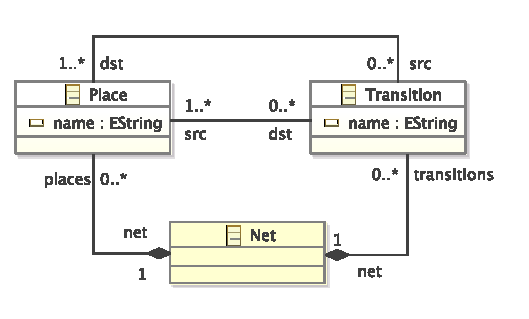
\includegraphics[scale=0.75]{petri_nets_step0.pdf}
  \caption{Original Petri nets metamodel.}
  \label{fig:original_mm}
\end{figure}

The evolved metamodel is shown in Figure~\ref{fig:evolved_mm}. \texttt{Place}s are connected to \texttt{Transition}s via instances of \texttt{PTArc}. Likewise, \texttt{Transition}s are connected to \texttt{Place}s via \texttt{TPArc}. Both \texttt{PTArc} and \texttt{TPArc} inherit from \texttt{Arc}, and therefore can be used to specify a \texttt{weight}.

\begin{figure}[htbp]
  \centering
  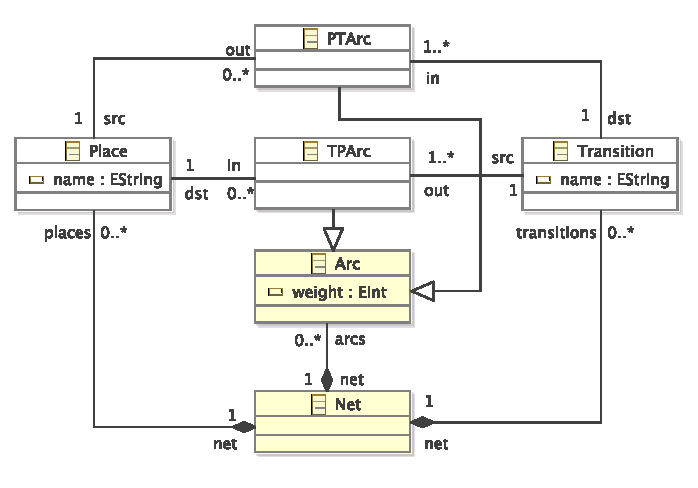
\includegraphics[scale=0.75]{petri_nets_step1.pdf}
  \caption{Evolved Petri nets metamodel.}
  \label{fig:evolved_mm}
\end{figure}

Models that were consistent with the original metamodel may not be consistent with the evolved metamodel. For example, \texttt{Transition} objects can no longer define values for \texttt{src} and \texttt{dst} features, and must define at least one value for the \texttt{in} and \texttt{out} features.

The migration strategy for this evolution varies when specified in ATL, COPE and Flock, largely due to the differences in the way in which each approach initialises migrated models. When specified in ATL, migration must copy values from original to migrated model, as shown on lines 5-6, 12 and 20 of Listing~\ref{lst:quantitive_etl}. When using COPE, values contained in slots that no longer correspond to features in the migrated metamodel must be unset, as shown on lines 2, 9 and 18-19 of Listing~\ref{lst:quantitive_cope}. Finally, Flock initialises the migrated model by copying values only for those features that remain unchanged in the migrated model. Consequently, no explicit copying or unsetting is required in Listing~\ref{lst:quantitive_flock}; the migration strategy manipulates only metafeatures that do not exist in the evolved metamodel (\texttt{Transition\#src} and \texttt{Transition\#dst}) and the new metaclasses, \texttt{TPArc} and \texttt{PTArc}.

\begin{lstlisting}[basicstyle=\ttfamily\footnotesize, flexiblecolumns=true, numbers=left, nolol=true, caption=Petri nets model migration in ETL, label=lst:quantitive_etl, language=ETL, tabsize=2]
rule Net2Net
  transform o : Original!Net
  to        m : Migrated!Net {

  m.places      := o.places.equivalent();
  m.transitions := o.transitions.equivalent();
}

rule Place2Place
  transform o : Original!Place
  to        m : Migrated!Place {

  m.name := o.name;
}

rule Transition2Transition
  transform o : Original!Transition
  to        m : Migrated!Transition {

  m.name := o.name;

  for (source in o.src) {
    var arc := new Migrated!PTArc;
    arc.src := source.equivalent();
    arc.dst := m;
    arc.net := o.net.equivalent();
  }

  for (destination in o.dst) {
    var arc := new Migrated!TPArc;
    arc.src := m;
    arc.dst := destination.equivalent();
    arc.net := o.net.equivalent();
  }
}
\end{lstlisting}


\begin{lstlisting}[basicstyle=\ttfamily\footnotesize, flexiblecolumns=true, numbers=left, nolol=true, caption=Petri nets model migration in COPE, label=lst:quantitive_cope, language=Java, tabsize=2]
for (transition in Transition.allInstances) {
  for (source in transition.unset('src')) {
    def arc = petrinets.PTArc.newInstance()
    arc.src = source
    arc.dst = transition
    arc.net = transition.net
  }

  for (destination in transition.unset('dst')) {
    def arc = petrinets.TPArc.newInstance() 
    arc.src = transition
    arc.dst = destination
    arc.net = transition.net
  }
}

for (place in Place.allInstances) {
  place.unset('src')
  place.unset('dst')
}
\end{lstlisting}


\begin{lstlisting}[basicstyle=\ttfamily\footnotesize, flexiblecolumns=true, numbers=left, nolol=true, caption=Petri nets model migration in Flock, label=lst:quantitive_flock, language=Flock, tabsize=2]
migrate Transition {
  for (source in original.src) {
    var arc := new Migrated!PTArc;
    arc.src := source.equivalent();
    arc.dst := migrated;
    arc.net := original.net.equivalent();
  }

  for (destination in original.dst) {
    var arc := new Migrated!TPArc;
    arc.src := migrated;
    arc.dst := destination.equivalent();
    arc.net := original.net.equivalent();
  }
}
\end{lstlisting}

With regard to the way in which they initialise the migrated model, COPE and ATL are opposites. The former initialises an exact copy of the original model, and so unset operations must be used when the value of a feature should not have been copied. By contrast, the latter initialises an empty model, and so explicit assignment operations must be used to copy values from original to migrated model for each feature that is not affected by the metamodel evolution.

This difference explains almost all of the results shown in Table~\ref{tab:model_operations_results}. Firstly, because Flock requires no unsetting of affected model elements nor explicit copying of unaffected model elements, less model operations are used when specifying a migration strategy with Flock than is used when specifying the same migration strategy with COPE or with ATL. Secondly, in most of the fifteen examples, there are more features unaffected by metamodel evolution than affected. Consequently, specifying model migration with ATL for the examples shown in Table~\ref{tab:model_operations_results} requires more model operations than in COPE. In the FPTC Connections and Ref Inline Class examples, the opposite is true (i.e. more features are affected by metamodel evolution than affected) and so encoding the migration strategy with ATL requires less model operations than with COPE. 


\subsubsection{Side-Effects during Initialisation}
The measurements observed for one example, Change R to C, cannot be explained by the difference in copying strategy. Instead, the way in which models are initialised by the migration languages must be considered. When a reference feature is changed to a containment reference during metamodel evolution, constructing the migrated model by starting from the original model (as is the case with COPE and, when the feature is not renamed, also Flock) can have side-effects which complicate migration. For the examples in Table~\ref{tab:model_operations_results}, only Change R to C, discussed below, was affected by this phenomenon.

In the Change R to C example, a \texttt{System} initially comprises \texttt{Port}s and \texttt{Signature}s (Figure~\ref{fig:ref2cont_original_mm}). A \texttt{Signature} references any number of \texttt{ports}. The metamodel is to be evolved so that \texttt{Port}s can no longer be shared between \texttt{Signature}s.

\begin{figure}[htbp]
  \centering
  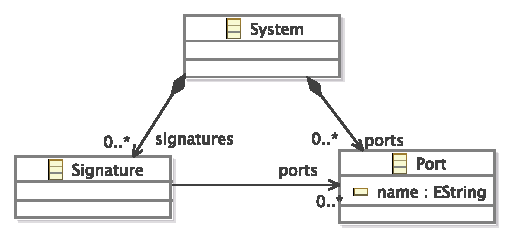
\includegraphics[scale=0.75]{change_ref_to_cont_before.pdf}
  \caption{Original metamodel.}
  \label{fig:ref2cont_original_mm}
\end{figure}

The evolved metamodel is shown in Figure~\ref{fig:ref2cont_evolved_mm}. \texttt{Signature}s now contain - rather than reference - \texttt{Port}s. Consequently, the \texttt{ports} feature of \texttt{System} is no longer required and is removed.

\begin{figure}[htbp]
  \centering
  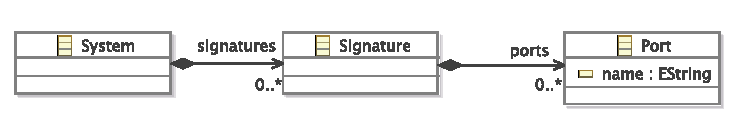
\includegraphics[scale=0.75]{change_ref_to_cont_after.pdf}
  \caption{Evolved metamodel.}
  \label{fig:ref2cont_evolved_mm}
\end{figure}

The migration strategy is straightforward in ATL: for each \texttt{Signature} in the original model, each member of the \texttt{ports} feature is cloned and added to the \texttt{ports} feature of the equivalent \texttt{Signature}.

\begin{lstlisting}[basicstyle=\ttfamily\footnotesize, flexiblecolumns=true, numbers=left, nolol=true, caption=Change R to C model migration in ATL, label=lst:ref2cont_atl, language=ATL, tabsize=2]
rule System2System
	transform old : Old!System
	to        s   : New!System {
	
	s.signatures := old.signatures.equivalent();
}

rule Signature2Signature
	transform old : Old!Signature
	to        s   : New!Signature {
	
	for (port in old.ports) {
		var clone := new New!Port;
		clone.name := port.name;
		s.ports.add(clone);
	}
}
\end{lstlisting}

In Flock and COPE, migration is less straightforward because, during migration, the value of a containment reference (\texttt{Signature\#ports}) is set automatically by the migration strategy execution engine. When a containment reference is set, the contained objects are removed from their previous containment reference (i.e. setting a containment reference can have side-effects). Therefore, in a \texttt{System} where more than one \texttt{Signature} references the same \texttt{Port}, the migrated model cannot be formed by copying the contents of \texttt{Signature\#ports} from the original model. Attempting to do so causes each \texttt{Port} to be contained only in the last referencing \texttt{Signature} that was copied.

In COPE, the containment nature of the reference is not enforced until after the migration strategy is executed. Hence, the migration strategy can be specified by unsetting the contents of the \texttt{ports} reference (line 4 of Listing~\ref{lst:ref2cont_cope}), and creating a copy of each referenced \texttt{Port} (lines 5-7 of Listing~\ref{lst:ref2cont_cope}). Unlike the ATL migration strategy, the COPE migration strategy ports are cloned in the same model as the original port. Consequently, the COPE migration strategy must either only clone ports that are referenced by more than one signature or clone every referenced port, but delete all of the original ports. The latter approach requires 2 more model operations (to populate and delete the original ports) than the former (shown in Listing~\ref{lst:ref2cont_cope}).

\begin{lstlisting}[basicstyle=\ttfamily\footnotesize, flexiblecolumns=true, numbers=left, nolol=true, caption=Change R to C model migration in COPE, label=lst:ref2cont_cope, language=COPE, tabsize=2]
def contained = []

for(signature in refactorings_changeRefToCont.Signature.allInstances) {
  for(port in signature.ports)) {
	  // when more than one Signature references this port
	  if (contained.contains(port)) {
      def clone = Port.newInstance()
      clone.name = port.name
      signature.ports.add(clone)
      signature.ports.remove(port)
		} else {
			contained.add(port)
		}
  }
}

for(port in refactorings_changeRefToCont.Port.allInstances) {
	if (not refactorings_changeRefToCont.Signature.allInstances.any { it.ports.contains(port) }) {
	  	port.delete()
	}
}
\end{lstlisting}

In Flock, the containment nature of the reference is enforced when the migrated model is initialised. Because changing the contents of a containment reference can have side-effects, a \texttt{Port} that appears in the \texttt{ports} reference of a \texttt{Signature} in the original model may not have been automatically copied to the \texttt{ports} reference of the equivalent \texttt{Signature} in the migrated model during initialisation. Consequently, the migration strategy must check the \texttt{ports} reference of each migrated \texttt{Signature}, cloning only those \texttt{Port}s that have not be automatically copied during initialisation (see line 3 of Listing~\ref{lst:ref2cont_flock}).

\begin{lstlisting}[basicstyle=\ttfamily\footnotesize, flexiblecolumns=true, numbers=left, nolol=true, caption=Change R to C model migration in Flock, label=lst:ref2cont_flock, language=Flock, tabsize=2]
migrate Signature {
	for (port in original.ports) {
		if (migrated.ports.excludes(port.equivalent())) {
			var clone := new Migrated!Port;
			clone.name := port.name;
			migrated.ports.add(clone);
		}
	}
}

delete Port when: not Original!Signature.all.exists(s|s.ports.includes(original))
\end{lstlisting}


The COPE and Flock migration strategies must also remove any \texttt{Port}s which are not referenced by any \texttt{Signature} (lines 17-21 of Listing~\ref{lst:ref2cont_cope}, and line 11 of Listing~\ref{lst:ref2cont_flock} respectively), whereas the ATL migration strategy, which initialises any empty migrated model, does not copy unreferenced \texttt{Port}s.

When a non-containment reference is changed to a containment reference, a Flock migration strategy requires one more more model operation than the equivalent ATL migration strategy: to delete model elements that are not contained in any instance of the containment reference (line 11 of Listing~\ref{lst:ref2cont_flock}). A COPE migration strategy requires three more model operations than the equivalent ATL migration strategy: one to delete model elements that are not contained in any instance of the containment reference (lines 17-21 of Listing~\ref{lst:ref2cont_cope}), one to dereference model elements that have already been cloned (line 10 of Listing~\ref{lst:ref2cont_cope}), and one to mark a model element as contained (line 12 of Listing~\ref{lst:ref2cont_cope}).  In the example considered here, the ATL migration strategy requires one more model operation than the Flock and COPE migration strategies (to copy the contents of System\#signature features from original to migrated model), due to the difference in copying strategy. This leads to the result shown in Table~\ref{tab:model_operations_results}: the Flock and ATL migration strategies have an equal number of model operations, while the COPE migration strategy has two more.


\subsection{Summary}
This section has compared the model migration languages

- Make clear the contribution: no other research has attempted to compare model migration languages. It's not clear how it should be done. This is a start. 
- Not trying to argue that the figures are statistically significant. Just an approximation of what we're trying to measure.
- Extensions: measure cyclomatic complexity, etc




\section{Discussion}
% We will discuss the limitations of our work, using for context the feedback of users, reviews of publications and scenarios from the case study discussed in Section~\ref{subsubsec:case_study}

\subsection{Threats to validity}



\section{Dissemination / Reception / ??}

\subsection{Publications}
% Publication in academic journals, and at international conferences and workshops ensure that our work is reviewed by experts, and is well-established and communicated in our field of research. So far, I have been the primary author for publications at one international conference (\cite{rose08hutn}), one European conference (\cite{rose08egl}), and one workshop (\cite{rose09patterns}). The first was published at MoDELS/UML, the leading international conference on model-driven engineering, in a year when it had a record number of submissions (274, 20\% acceptance), and has been nominated by HISE for the annual departmental award for best paper by a research student.

% We will submit our work to software evolution conferences, as well as at model-driven engineering conferences. Doing so will allow us to assess the impact of our research for a broader audience.


\subsection{Delivery through Eclipse}
% The tools produced as part of our research have been and will continue to be released as part of the Epsilon project, a member of the research incubator for the Eclipse Modeling Project (EMP), arguably the most active MDE community at present. EMP's research incubator hosts a limited number of participants, selected through a rigorous process. Contributions made to the incubator undergo regular technical review.

% Contributing to Epsilon allows us to deliver our research to the growing community \cite{kolovos08thesis} of Epsilon users.
